% Reduced density matrix against reduced transition matrix.
% Tensor proportions follow carignano_tagliacozzo2025 (Fig. 10): large circles with heavy outlines,
% short thick bonds, saturated flat fills.
%
% Standalone: compiles to imgs/rdm_rtm.pdf.
% Inline:     with \usepackage{standalone}, % Reduced density matrix against reduced transition matrix.
% Tensor proportions follow carignano_tagliacozzo2025 (Fig. 10): large circles with heavy outlines,
% short thick bonds, saturated flat fills.
%
% Standalone: compiles to imgs/rdm_rtm.pdf.
% Inline:     with \usepackage{standalone}, % Reduced density matrix against reduced transition matrix.
% Tensor proportions follow carignano_tagliacozzo2025 (Fig. 10): large circles with heavy outlines,
% short thick bonds, saturated flat fills.
%
% Standalone: compiles to imgs/rdm_rtm.pdf.
% Inline:     with \usepackage{standalone}, % Reduced density matrix against reduced transition matrix.
% Tensor proportions follow carignano_tagliacozzo2025 (Fig. 10): large circles with heavy outlines,
% short thick bonds, saturated flat fills.
%
% Standalone: compiles to imgs/rdm_rtm.pdf.
% Inline:     with \usepackage{standalone}, \input{imgs/rdm_rtm}.
\documentclass[tikz,border=3pt]{standalone}
\usepackage{amsmath,amssymb,braket}
\usetikzlibrary{arrows.meta}

\definecolor{tnL}{RGB}{243,116,63}
\definecolor{tnR}{RGB}{60,110,150}
\definecolor{tnLl}{RGB}{250,190,150}

\newcommand{\DX}{1.12}    % centre-to-centre, about 1.7 circle diameters
\newcommand{\DY}{0.60}    % half the row separation
\newcommand{\ST}{0.66}    % dangling leg: circle radius 0.33 plus a visible stub

\begin{document}
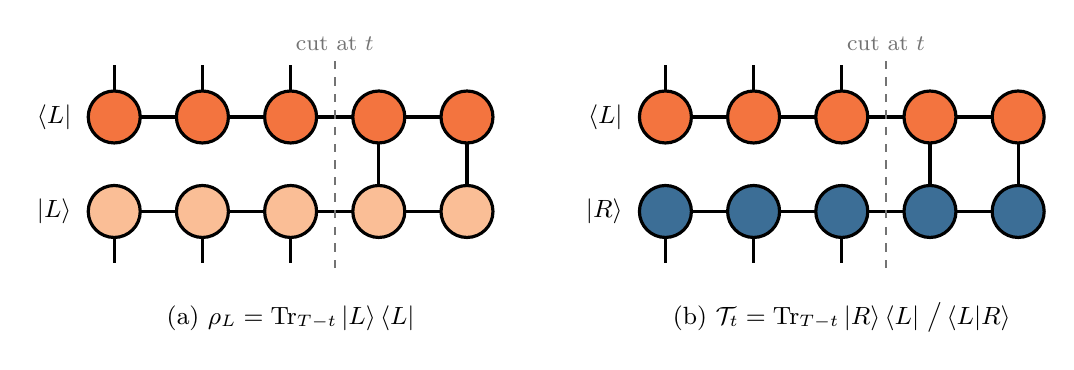
\begin{tikzpicture}[
    bond/.style={draw=black, line width=1.15pt},
    T/.style={circle, draw=black, line width=1.15pt, minimum size=6.6mm, inner sep=0pt},
    tag/.style={font=\small},
    idx/.style={font=\footnotesize},
  ]

  \newcommand{\panel}[4]{% #1 xshift, #2 top fill, #3 bottom fill, #4 caption
    \begin{scope}[xshift=#1]
      % virtual bonds along the temporal chain
      \draw[bond] (0,\DY)  -- ({4*\DX},\DY);
      \draw[bond] (0,-\DY) -- ({4*\DX},-\DY);
      % sites after the cut are traced: their physical legs contract with each other
      \foreach \i in {3,4} { \draw[bond] (\i*\DX,\DY) -- (\i*\DX,-\DY); }
      % sites before the cut keep their legs open
      \foreach \i in {0,1,2} {
        \draw[bond] (\i*\DX,\DY)  -- (\i*\DX,{\DY+\ST});
        \draw[bond] (\i*\DX,-\DY) -- (\i*\DX,{-\DY-\ST});
      }
      \foreach \i in {0,...,4} {
        \node[T, fill=#2] at (\i*\DX,\DY)  {};
        \node[T, fill=#3] at (\i*\DX,-\DY) {};
      }
      \draw[black!55, dashed, line width=0.7pt] ({2.5*\DX},{-\DY-0.72}) -- ({2.5*\DX},{\DY+0.72});
      \node[idx, black!55, anchor=south] at ({2.5*\DX},{\DY+0.72}) {cut at $t$};
      \node[tag] at ({2*\DX},{-\DY-1.35}) {#4};
    \end{scope}}

  \panel{0cm}{tnL}{tnLl}{(a) $\rho_L=\mathrm{Tr}_{T-t}\ket{L}\bra{L}$}
  \panel{7.0cm}{tnL}{tnR}{(b) $\mathcal{T}_t=\mathrm{Tr}_{T-t}\ket{R}\bra{L}\,\big/\,\langle L|R\rangle$}

  \node[tag, anchor=east] at (-0.42,\DY)       {$\bra{L}$};
  \node[tag, anchor=east] at (-0.42,-\DY)      {$\ket{L}$};
  \node[tag, anchor=east] at (6.58,\DY)        {$\bra{L}$};
  \node[tag, anchor=east] at (6.58,-\DY)       {$\ket{R}$};

\end{tikzpicture}
\end{document}
.
\documentclass[tikz,border=3pt]{standalone}
\usepackage{amsmath,amssymb,braket}
\usetikzlibrary{arrows.meta}

\definecolor{tnL}{RGB}{243,116,63}
\definecolor{tnR}{RGB}{60,110,150}
\definecolor{tnLl}{RGB}{250,190,150}

\newcommand{\DX}{1.12}    % centre-to-centre, about 1.7 circle diameters
\newcommand{\DY}{0.60}    % half the row separation
\newcommand{\ST}{0.66}    % dangling leg: circle radius 0.33 plus a visible stub

\begin{document}
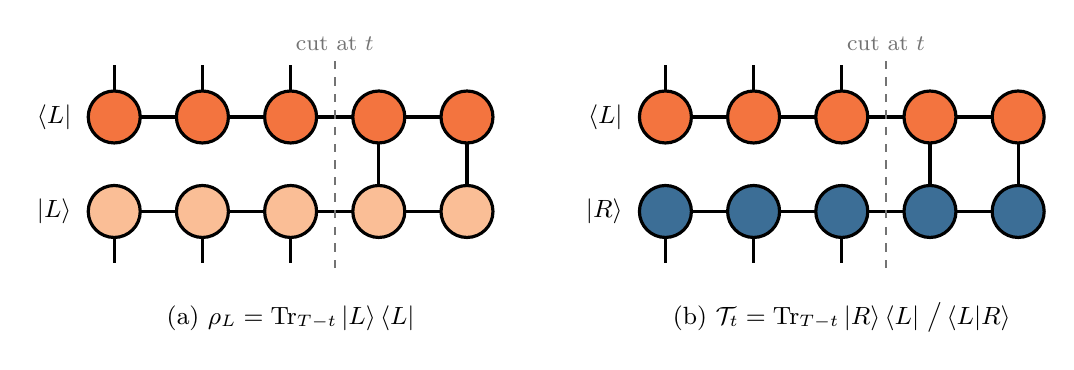
\begin{tikzpicture}[
    bond/.style={draw=black, line width=1.15pt},
    T/.style={circle, draw=black, line width=1.15pt, minimum size=6.6mm, inner sep=0pt},
    tag/.style={font=\small},
    idx/.style={font=\footnotesize},
  ]

  \newcommand{\panel}[4]{% #1 xshift, #2 top fill, #3 bottom fill, #4 caption
    \begin{scope}[xshift=#1]
      % virtual bonds along the temporal chain
      \draw[bond] (0,\DY)  -- ({4*\DX},\DY);
      \draw[bond] (0,-\DY) -- ({4*\DX},-\DY);
      % sites after the cut are traced: their physical legs contract with each other
      \foreach \i in {3,4} { \draw[bond] (\i*\DX,\DY) -- (\i*\DX,-\DY); }
      % sites before the cut keep their legs open
      \foreach \i in {0,1,2} {
        \draw[bond] (\i*\DX,\DY)  -- (\i*\DX,{\DY+\ST});
        \draw[bond] (\i*\DX,-\DY) -- (\i*\DX,{-\DY-\ST});
      }
      \foreach \i in {0,...,4} {
        \node[T, fill=#2] at (\i*\DX,\DY)  {};
        \node[T, fill=#3] at (\i*\DX,-\DY) {};
      }
      \draw[black!55, dashed, line width=0.7pt] ({2.5*\DX},{-\DY-0.72}) -- ({2.5*\DX},{\DY+0.72});
      \node[idx, black!55, anchor=south] at ({2.5*\DX},{\DY+0.72}) {cut at $t$};
      \node[tag] at ({2*\DX},{-\DY-1.35}) {#4};
    \end{scope}}

  \panel{0cm}{tnL}{tnLl}{(a) $\rho_L=\mathrm{Tr}_{T-t}\ket{L}\bra{L}$}
  \panel{7.0cm}{tnL}{tnR}{(b) $\mathcal{T}_t=\mathrm{Tr}_{T-t}\ket{R}\bra{L}\,\big/\,\langle L|R\rangle$}

  \node[tag, anchor=east] at (-0.42,\DY)       {$\bra{L}$};
  \node[tag, anchor=east] at (-0.42,-\DY)      {$\ket{L}$};
  \node[tag, anchor=east] at (6.58,\DY)        {$\bra{L}$};
  \node[tag, anchor=east] at (6.58,-\DY)       {$\ket{R}$};

\end{tikzpicture}
\end{document}
.
\documentclass[tikz,border=3pt]{standalone}
\usepackage{amsmath,amssymb,braket}
\usetikzlibrary{arrows.meta}

\definecolor{tnL}{RGB}{243,116,63}
\definecolor{tnR}{RGB}{60,110,150}
\definecolor{tnLl}{RGB}{250,190,150}

\newcommand{\DX}{1.12}    % centre-to-centre, about 1.7 circle diameters
\newcommand{\DY}{0.60}    % half the row separation
\newcommand{\ST}{0.66}    % dangling leg: circle radius 0.33 plus a visible stub

\begin{document}
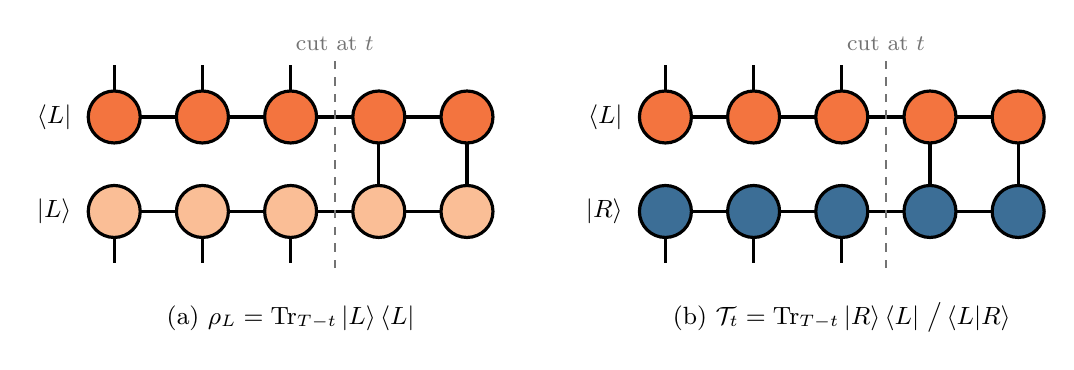
\begin{tikzpicture}[
    bond/.style={draw=black, line width=1.15pt},
    T/.style={circle, draw=black, line width=1.15pt, minimum size=6.6mm, inner sep=0pt},
    tag/.style={font=\small},
    idx/.style={font=\footnotesize},
  ]

  \newcommand{\panel}[4]{% #1 xshift, #2 top fill, #3 bottom fill, #4 caption
    \begin{scope}[xshift=#1]
      % virtual bonds along the temporal chain
      \draw[bond] (0,\DY)  -- ({4*\DX},\DY);
      \draw[bond] (0,-\DY) -- ({4*\DX},-\DY);
      % sites after the cut are traced: their physical legs contract with each other
      \foreach \i in {3,4} { \draw[bond] (\i*\DX,\DY) -- (\i*\DX,-\DY); }
      % sites before the cut keep their legs open
      \foreach \i in {0,1,2} {
        \draw[bond] (\i*\DX,\DY)  -- (\i*\DX,{\DY+\ST});
        \draw[bond] (\i*\DX,-\DY) -- (\i*\DX,{-\DY-\ST});
      }
      \foreach \i in {0,...,4} {
        \node[T, fill=#2] at (\i*\DX,\DY)  {};
        \node[T, fill=#3] at (\i*\DX,-\DY) {};
      }
      \draw[black!55, dashed, line width=0.7pt] ({2.5*\DX},{-\DY-0.72}) -- ({2.5*\DX},{\DY+0.72});
      \node[idx, black!55, anchor=south] at ({2.5*\DX},{\DY+0.72}) {cut at $t$};
      \node[tag] at ({2*\DX},{-\DY-1.35}) {#4};
    \end{scope}}

  \panel{0cm}{tnL}{tnLl}{(a) $\rho_L=\mathrm{Tr}_{T-t}\ket{L}\bra{L}$}
  \panel{7.0cm}{tnL}{tnR}{(b) $\mathcal{T}_t=\mathrm{Tr}_{T-t}\ket{R}\bra{L}\,\big/\,\langle L|R\rangle$}

  \node[tag, anchor=east] at (-0.42,\DY)       {$\bra{L}$};
  \node[tag, anchor=east] at (-0.42,-\DY)      {$\ket{L}$};
  \node[tag, anchor=east] at (6.58,\DY)        {$\bra{L}$};
  \node[tag, anchor=east] at (6.58,-\DY)       {$\ket{R}$};

\end{tikzpicture}
\end{document}
.
\documentclass[tikz,border=3pt]{standalone}
\usepackage{amsmath,amssymb,braket}
\usetikzlibrary{arrows.meta}

\definecolor{tnL}{RGB}{243,116,63}
\definecolor{tnR}{RGB}{60,110,150}
\definecolor{tnLl}{RGB}{250,190,150}

\newcommand{\DX}{1.12}    % centre-to-centre, about 1.7 circle diameters
\newcommand{\DY}{0.60}    % half the row separation
\newcommand{\ST}{0.66}    % dangling leg: circle radius 0.33 plus a visible stub

\begin{document}
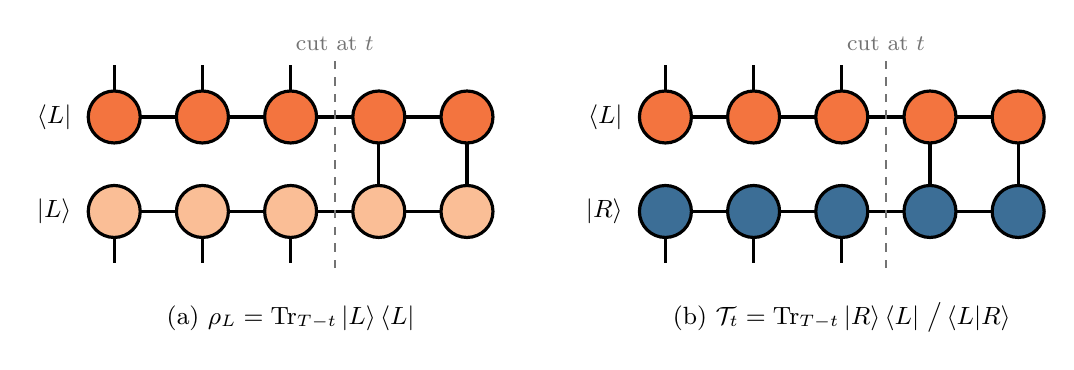
\begin{tikzpicture}[
    bond/.style={draw=black, line width=1.15pt},
    T/.style={circle, draw=black, line width=1.15pt, minimum size=6.6mm, inner sep=0pt},
    tag/.style={font=\small},
    idx/.style={font=\footnotesize},
  ]

  \newcommand{\panel}[4]{% #1 xshift, #2 top fill, #3 bottom fill, #4 caption
    \begin{scope}[xshift=#1]
      % virtual bonds along the temporal chain
      \draw[bond] (0,\DY)  -- ({4*\DX},\DY);
      \draw[bond] (0,-\DY) -- ({4*\DX},-\DY);
      % sites after the cut are traced: their physical legs contract with each other
      \foreach \i in {3,4} { \draw[bond] (\i*\DX,\DY) -- (\i*\DX,-\DY); }
      % sites before the cut keep their legs open
      \foreach \i in {0,1,2} {
        \draw[bond] (\i*\DX,\DY)  -- (\i*\DX,{\DY+\ST});
        \draw[bond] (\i*\DX,-\DY) -- (\i*\DX,{-\DY-\ST});
      }
      \foreach \i in {0,...,4} {
        \node[T, fill=#2] at (\i*\DX,\DY)  {};
        \node[T, fill=#3] at (\i*\DX,-\DY) {};
      }
      \draw[black!55, dashed, line width=0.7pt] ({2.5*\DX},{-\DY-0.72}) -- ({2.5*\DX},{\DY+0.72});
      \node[idx, black!55, anchor=south] at ({2.5*\DX},{\DY+0.72}) {cut at $t$};
      \node[tag] at ({2*\DX},{-\DY-1.35}) {#4};
    \end{scope}}

  \panel{0cm}{tnL}{tnLl}{(a) $\rho_L=\mathrm{Tr}_{T-t}\ket{L}\bra{L}$}
  \panel{7.0cm}{tnL}{tnR}{(b) $\mathcal{T}_t=\mathrm{Tr}_{T-t}\ket{R}\bra{L}\,\big/\,\langle L|R\rangle$}

  \node[tag, anchor=east] at (-0.42,\DY)       {$\bra{L}$};
  \node[tag, anchor=east] at (-0.42,-\DY)      {$\ket{L}$};
  \node[tag, anchor=east] at (6.58,\DY)        {$\bra{L}$};
  \node[tag, anchor=east] at (6.58,-\DY)       {$\ket{R}$};

\end{tikzpicture}
\end{document}
